\section{Vorlesung 05.04.2016}
\subsection{Aktionspotential}
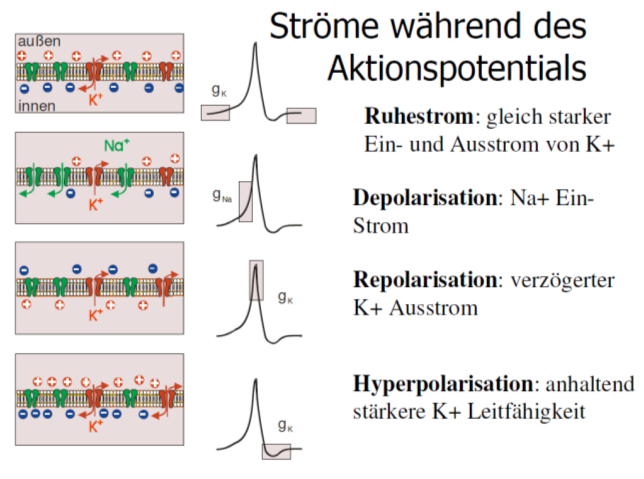
\includegraphics[width=1\textwidth]{lectures/160405/pix/aktionspotential.png}

Aktionspotentiale werden "aktiv" fortgeleitet:
\begin{itemize}
	\item schnell
	\item ohne Abschwächung (Leitungswiderstand!)
	\item ohne $"$Informationsverlust" (nur innerhahlb eines Neurons möglich, von Neuron zu Neuron \textbf{muss} es durch AD-Wandlung Verluste geben)
	\item in eine Richtung
\end{itemize}

 - Durch Refrakterzeit (Erholungszeit) ist Richtung der Weiterleitung eindeutig

\subsubsection{SNARE-Proteine und ihre Gifte}
\begin{itemize}
	\item SNARE-Komplexe katalysieren bei der Fusion von biologischen Membranen den Transport von small molecules, beispielsweise bei einer Exozytose in den synaptischen Spalt
	\item SNAREs als Ziel von Neurotoxinen (bakterielle Gifte):
		\begin{itemize}
			\item spalten SNARE-Proteine, wodurch die Vesikelfusion und somit die Transmitterfreisetzung verhindert wird
			\item Botulinum Toxine $\rightarrow$ Fleischvergiftung, Tod durch Lähmung der Atmung
			\item Tetanus Toxin
		\end{itemize}
\end{itemize}

\subsubsection{Neurotransmitter}
\textbf{Acetylcholin} als wichtigster Neurotransmitter\\
weitere:
\begin{itemize}
	\item biogene Amine: Adrenalin, Serotonin
	\item Aminosäuren: GABA (Gamma-Amino-Butteracid), Glycin, Glutamat
	\item Peptide: Opioide, Substanz P, Insulin
	\item gasförmige Transmitter: Stickoxid, Kohlenmonoxid
\end{itemize}

\subsection{chemische Synapse}
\begin{itemize}
	\item synaptische Spalt: 20 - 40 nm
	\item präsynaptische Zelle mit Vesikeln setzt Botenstoffe (Neurotransmitter) frei, der durch den synaptischen Spalt zur postsynaptischen Zelle diffundiert und dort an spezifische Rezeptormoleküle bindet
	\item Menge des freigesetzten Transmitters abhängig von der Zahl der einlaufenden Aktionspotentiale
	\item chemische Synapsen sind gleichgerichtet (Leitung in nur eine Richtung) und arbeite mit einer Zeitverzögerung von ca. 1 ms
\end{itemize}
\newpage
zwei Arten von Rezeptormolekülen:
\begin{enumerate}
	\item Ionotrope Rezeptoren:
		\begin{itemize}
			\item Ionenkanäle
			\item schnelle, im Millisekundenbereich liegende Änderung des Membranpotentials der postsynaptischen Zelle
		\end{itemize}
	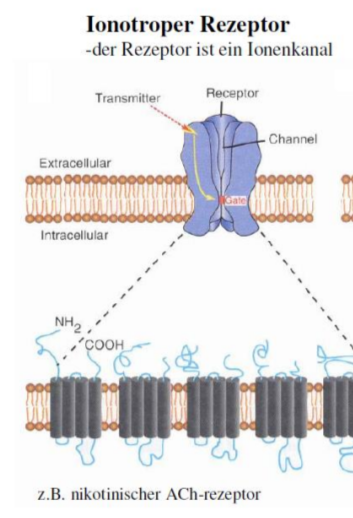
\includegraphics[width=0.75\textwidth]{lectures/160405/pix/ionotrop.png}\newpage
	\item metabotrope Rezeptoren:
		\begin{itemize}
			\item lösen Signalkaskaden aus
			\item langsame Änderung des Membranpotentials im hunderte Milli- und Sekundenbereich
			\item Bildung von intrazellulären Botenstoffen (secondary messenger)
		\end{itemize}
	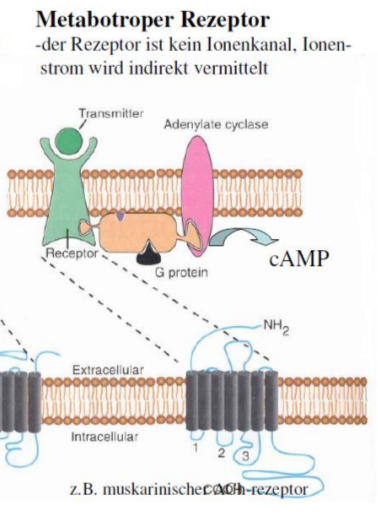
\includegraphics[width=0.75\textwidth]{lectures/160405/pix/metabotrop.png}\newpage
\end{enumerate}

\textbf{Inhibitorische postsynaptische Potentiale (IPSP)}\\
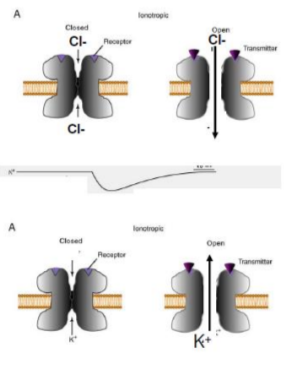
\includegraphics[width=0.5\textwidth]{lectures/160405/pix/ipsp.png}

\textbf{Exzitatorische postsynaptische Potentiale (EPSP) von ionotropen und metabotropen Rezeptoren}\\
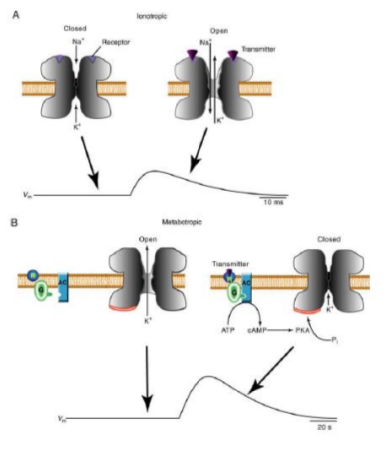
\includegraphics[width=0.65\textwidth]{lectures/160405/pix/epsp.png}

Ob ein NT erregend (exzitatorisch) oder hemmend (inhibitorisch) wirkt, hängt ausschließlich von der Art der postsynaptischen Rezeptormolekülen ab:
\begin{itemize}
	\item erregend: Bildung eines EPSPs
	\item hemmend: Bildung eines IPSPs
\end{itemize}

Eine Nervenzelle kann mehr als einen Transmitter freisetzen (oft klassischer Transmitter und ein bis mehrerer Co-Transmitter)
\\\\
\textbf{Verrechnung (Intergration) an Synapsen}\\
 - Addition und Subtraktion\\\\
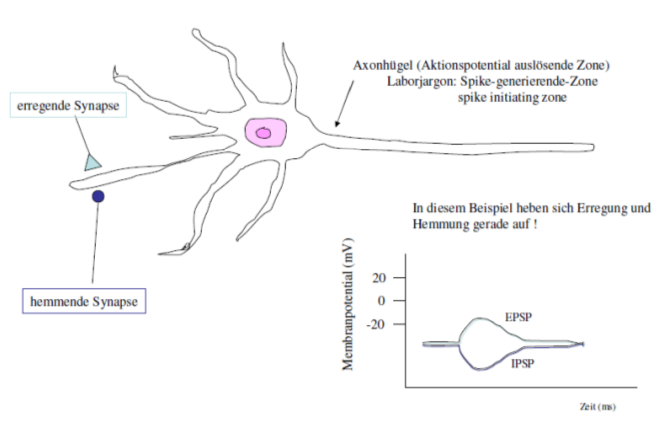
\includegraphics[width=1\textwidth]{lectures/160405/pix/calculation.png}
\\\\
\underline{räumliche Summation:} EPSPs/IPSPs verschiedener Synapsen, die z.B. an einem Dendritenbaum ansetzen, werden in der postsynaptischen Zelle zu jedem Zeitpunkt addiert\\

\underline{zeitliche Summation:} Die in einer Präsynapse zeitlich kurz aufeinanderfolgenden Aktionspotentiale lösen in der postsynaptischen Zeller EPSPs/IPSPs aus, welche addiert werden.
Für die Integration sind die passiven elektrischen Eigenschaften (Kabeleigenschaften) des postsynaptischen Neurons sehr wichtig.\\\\

\textbf{Synaptische Potentiale sind abgestuft (graduiert) $\Rightarrow$ neben den Aktionspotentialen die zweite Form der Erregung im Nervensystem}
\\\\
\textbf{Präsynaptische Hemmung an Synapsen}\\
Das präsynaptische Neuron wird durch Freisetzung eines Transmitters (vorwiegend GABA oder Glycerin) gehemmt und damit wird die Freisettzung des Transmitters aus der Präsynapse verhindert.\\\\
Ein Mechanismus, der z.B. die Axonterminale von Sinneszellen differenziert hemmen kann und damit die sensorischen Signale unterdruckt.
\\\\
\textbf{Bahnung (Fazilitation) an Synapsen}\\
\underline{Homosynaptische Bahnung:} EPSP-Größe nimmt zu, wenn präsynaptische Aktionspotentiale in einer Salve kommen
\\\\
\underline{Heterosynaptische Bahnung:} Durch Transmitterfreisetzung aus einem dritten Neuron (Neuromodulator) wird die synaptische Übertragung gesteigert\\

\textbf{Synaptische Depression}
\begin{itemize}
	\item Abnahme des postsynaptischen Potentials bei rascher Wiederholung des präsynaptischen Eingangs
	\item Ausschließlich oder überwiegend ein postsynaptisches Phänomen
\end{itemize}

\textbf{Modulation von Synapsen}
\begin{itemize}
	\item prä- und postsynaptische Zelle werden durch NTs (Neuromodulatoren) von drittem Neuron beeinflusst
	\item hat selbst keine rasche Wirkung auf Neurone $\rightarrow$ normale Übertragung wird verändert, z.B. effizienter
	\item Neuromodulatoren sind häufig biogene Amine (Dopamin, Serotonin)
\end{itemize}

\textbf{Lern und Gedächtnisbildung beruht auf bestimmten Formen der aktivitätsabhängigen (assoziativen) Neuromodulation}